\documentclass[a4paper,12pt]{article}
\usepackage[greek]{babel}
\usepackage{fontspec}
\usepackage{xunicode}
\usepackage{xltxtra}
\setmainfont{Linux Libertine O}
\usepackage{graphicx}
\usepackage{hyperref}
\usepackage{listings}
\usepackage{color}
\usepackage{titlesec}
\usepackage{geometry}
\usepackage{enumitem}

\geometry{margin=2.5cm}

\title{\textbf{Αναφορά Ανάπτυξης Project: The Best Banking System}}
\author{Ομάδα Φοιτητών Τμήματος Μηχανικών Πληροφορικής ΔΙΠΑΕ Σερρών \\[0.5em]
\textbf{Μάριο Βέλα} \\ 
\textbf{Θεοδώσης Στάμογλου} \\ 
\textbf{Άγγελος Κουρουγένης}}
\date{Μάιος 2025}

\begin{document}

\maketitle

\tableofcontents
\newpage

\section{Εισαγωγή και Motivation}
Το project \textbf{The Best Banking System} είναι μια εκπαιδευτική αλλά και πλήρως λειτουργική προσομοίωση ενός τραπεζικού πληροφοριακού συστήματος. Η εφαρμογή καλύπττει βασικές και προηγμένες λειτουργίες μιας σύγχρονης ηλεκτρονικής τράπεζας.

Το πρόβλημα που αντιμετωπίζει είναι η ανάγκη για ασφαλή, επεκτάσιμη και εκπαιδευτική πλατφόρμα διαχείρισης λογαριασμών και συναλλαγών με έμφαση στην προστασία του χρήστη.

Η επιλογή του αντικειμένου έγινε με γνώμονα:
\begin{itemize}[label=\textbullet]
    \item την ενίσχυση δεξιοτήτων στον αντικειμενοστραφή προγραμματισμό,
    \item τη χρήση τεχνολογιών ασφάλειας όπως OTP και hash passwords,
    \item την επαφή με real-world concepts όπως τόκοι, verification και επικοινωνία με email.
\end{itemize}

\section{Στόχοι και Εύρος του Project}
\subsection*{Κύριοι στόχοι}
\begin{itemize}[label=\textbullet]
    \item Ανάπτυξη πλήρους C++ backend για λογαριασμούς και συναλλαγές
    \item Επαλήθευση χρηστών μέσω email OTP
    \item Αποστολή HTML email με πληροφορίες τόκων
    \item Αυτόματη εφαρμογή τόκων 2 φορές το χρόνο
    \item Διαχείριση στοιχείων χρήστη με προστασία δεδομένων
\end{itemize}

\subsection*{Επέκταση και Εύρος}
\begin{itemize}[label=\textbullet]
    \item Σύνδεση C++ με Python scripts μέσω system calls
    \item Εφαρμογή πολιτικής επαναπροσπάθειας και κλειδώματος λογαριασμών
    \item Δυνατότητα πολλαπλών μενού για διαχείριση (User, Account Management, Transactions)
    \item Υποστήριξη αρχείων `.txt` για αποθήκευση χωρίς βάση δεδομένων
    \item Modular design με δυνατότητα μελλοντικής σύνδεσης με Web Interface
\end{itemize}

\section{Αρχιτεκτονική Συστήματος}
\subsection*{Επισκόπηση}
Το σύστημα αποτελείται από 3 βασικά στρώματα:
\begin{itemize}[label=\textbullet]
    \item \textbf{Εφαρμογή C++:} Κύριος κορμός λογικής και διαχείρισης δεδομένων
    \item \textbf{Scripts Python:} Αποστολή OTP και ενημερωτικών email (SMTP/SSL)
    \item \textbf{Αρχεία δεδομένων:} Αποθήκευση λογαριασμών και ιστορικού
\end{itemize}

\newpage
\thispagestyle{empty}
\newgeometry{left=0cm, right=0cm, top=0cm, bottom=0cm}
\begin{figure}
    \centering
    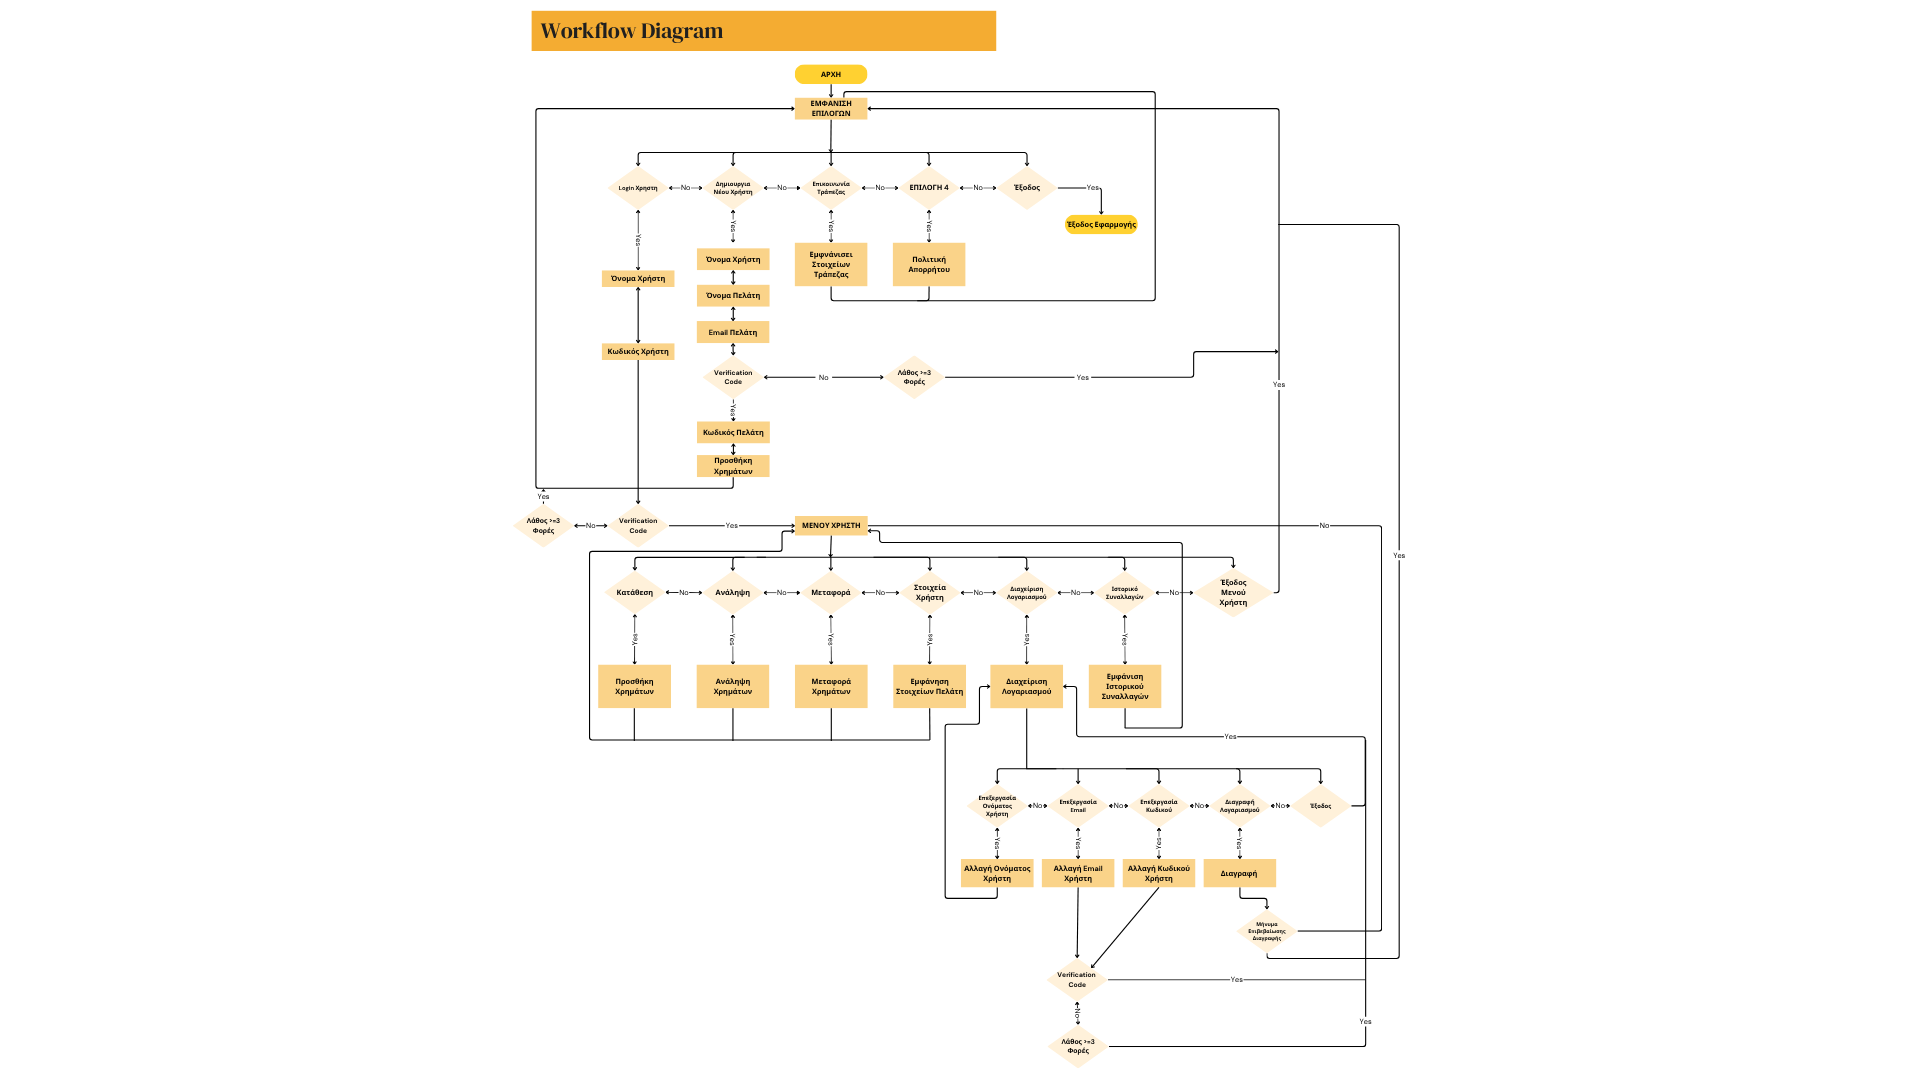
\includegraphics[width=\paperwidth,height=\paperheight,keepaspectratio]{Workflow_Diagram.png}
    \caption{Workflow Diagram}
\end{figure}
\restoregeometry
\newpage

\section{Τεχνολογίες και Βιβλιοθήκες}
\subsection*{Γλώσσες και Εργαλεία}
\begin{itemize}[label=\textbullet]
    \item C++ για αντικειμενοστραφή προγραμματισμό
    \item Python 3 για email handling
    \item G++ compiler για build
    \item Git για version control
\end{itemize}

\subsection*{Βιβλιοθήκες}
\textbf{C++:} \texttt{vector, string, fstream, iomanip, regex, chrono, map, random} \\ 
\textbf{Python:} \texttt{smtplib, ssl, email.mime} 

\section{Κώδικας και Υλοποίηση}
Η υλοποίηση βασίζεται σε:
\begin{enumerate}[label=\arabic*.]
    \item \textbf{banking\_system.cpp:} Κύριο αρχείο με κλάσεις \texttt{BankAccount}, \texttt{Transaction}, και \texttt{BankSystem}
    \item \textbf{send\_otp\_email.py:} Αποστολή OTP σε πραγματικό χρόνο
    \item \textbf{send\_interest\_info\_email.py:} HTML ενημέρωση για τους τόκους
\end{enumerate}

\subsection*{Σημαντικά χαρακτηριστικά}
\begin{itemize}[label=\textbullet]
    \item Έλεγχος εγκυρότητας username και password με regex
    \item Δημιουργία μοναδικού λογαριασμού με prefix-based αριθμούς
    \item Ενσωμάτωση 2FA με OTP και χρονικό περιορισμό
    \item Υπολογισμός τόκων (3\%) και προσθήκη σε ισολογισμό
    \item Καταγραφή συναλλαγών με timestamp και file output
\end{itemize}

\section{Αποτελέσματα και Demo}
\subsection*{Πραγματοποιημένα Features}
\begin{itemize}[label=\textbullet]
    \item Εγγραφή χρήστη με OTP (έλεγχος σε πραγματικό Gmail)
    \item Δημιουργία ασφαλών συναλλαγών
    \item Ιστορικό συναλλαγών ανά χρήστη
    \item Δομή μενού για ενίσχυση UX
    \item Μηχανισμός κλειδώματος λογαριασμού σε περίπτωση επαναλαμβανόμενης αποτυχίας
\end{itemize}

\subsection*{Έλεγχοι \& Test Cases}
\begin{itemize}[label=\textbullet]
    \item Εσφαλμένοι κωδικοί: 3 προσπάθειες και κλείδωμα
    \item OTP λήγει μετά από 60 δευτερόλεπτα
    \item Το email επιβεβαιώνεται πριν δημιουργηθεί λογαριασμός
    \item Εφαρμογή τόκων
\end{itemize}

\section{Σύγκριση με Κώδικα από AI}
\textbf{Πλεονεκτήματα Χειροκίνητης Ανάπτυξης:}
\begin{itemize}[label=\textbullet]
    \item Απόλυτος έλεγχος σε κάθε συνάρτηση και class
    \item Τεκμηρίωση, επεξήγηση, debugging και καλύτερη κατανόηση
    \item Δυνατότητα refactor και modular επεκτασιμότητας
\end{itemize}

\textbf{Προβλήματα AI-generated code:}
\begin{itemize}[label=\textbullet]
    \item Αγνοούνται corner cases
    \item Μη αξιόπιστη διαχείριση σφαλμάτων
    \item Δεν ακολουθεί απαραίτητα design principles
\end{itemize}

\section{Συμπεράσματα και Lessons Learned}
\begin{itemize}[label=\textbullet]
    \item Η συνεργασία γλωσσών (C++ με Python) μπορεί να γίνει ομαλά με καλό σχεδιασμό
    \item Η ασφαλής αυθεντικοποίηση είναι εφικτή χωρίς βάση δεδομένων
    \item Τα HTML email βελτιώνουν την εμπειρία χρήστη και αξιοπιστία
    \item Ο modular σχεδιασμός βοηθά στο testing και future-proofing
    \item Το σύστημα αποτελεί καλή βάση για πλήρες web banking platform
\end{itemize}

\section{Μελλοντικές Κατευθύνσεις}
\begin{itemize}[label=\textbullet]
    \item Δημιουργία Web Interface με Flask ή React
    \item Εγκατάσταση SQLite για πιο σταθερή αποθήκευση δεδομένων
    \item Υποστήριξη IBAN validation
    \item Role-based access για admins/users
    \item Αποστολή ειδοποιήσεων για ύποπτες συναλλαγές
\end{itemize}

\end{document}
